% ------------------------------------------------------------------------ %
% !TEX encoding = UTF-8
% !TEX TS-program = pdflatex
% !TEX root = ../Project.tex
% !TEX spellcheck = en-EN
% ------------------------------------------------------------------------ %
%
% ------------------------------------------------------------------------ %
% 	CHAPTER TITLE
% ------------------------------------------------------------------------ %
%
\chapter{Specific Requirements}
%
\label{cap:specificrequirements}
%

\section{Functional requirements}
The aim of the system is to give the user the following functionalities, arranged in sections:
\begin{itemize}
\item	Registration process:
\begin{enumerate}
\item the application will provide a registration process;
\item users can access to the functionalities provided by the system if and only if they register to it;
\item there are not users with privileges, every registered user can access to the same features of the other ones and the system is safe even without supervisors;
\item all data will be stored on the Travlendar+ server to backup user information and to allow it to be shared on different user’s devices.
\end{enumerate}
\item	Initial settings, always adjustable:
\begin{itemize}
\item set user personal information: 
\begin{enumerate}
	\setcounter{enumi}{4}
\item google account to synchronize calendar and maps;
\item house location, work location, new location;
\item default location to reach after appointments, to be chosen between the favourites (usually home);
\item user break times and guaranteed amount of time to keep free from trips in every break to have lunch or another dynamic event;
\item time of the day after which bike (owned or shared) and public transports will not be considered anymore in planning the trip.
\end{enumerate} 
\item set desired user transport means: 
\begin{enumerate}
  \setcounter{enumi}{9}
\item car possession, bike possession; 
\item car sharing account(s), bike sharing account(s);
\item public and private transports (possibility to insert season ticket);
\item maximum walking distance (to destination or sharing vehicle).
\end{enumerate}
\end{itemize}

\item	Scheduled event creation: 
\begin{enumerate}
  \setcounter{enumi}{13}
\item set day(s);
\item set time of beginning and end;
\item set location.
\end{enumerate}

\item	Calendar consultation and edit:
\begin{enumerate}
  \setcounter{enumi}{16}
\item see future scheduled events and meetings;
\item modify events previously added.
\end{enumerate}


\item	Planned trips consultation and edit:
\begin{enumerate}
  \setcounter{enumi}{18}
\item	desire to minimize carbon footprint;
\item	choose between any other trip possibilities in case the one recommended by Travlendar+ is not suitable;
\item	purchase tickets for public transports before the trip;
\item	presence of passengers;
\item	show the best travel option selected by the app on various factors;
\item	consult the map showing the best route to reach the destination, the sharing vehicle or the public transport stop.
\end{enumerate}

\item	On arrival of scheduled meeting:
\begin{enumerate}
  \setcounter{enumi}{24}
\item	notification service informing the user he needs to leave to the next meeting in half an hour;
\item	notification service telling the user the time to leave to the next meeting has come;
\item	alert the user of trips’ changes between the first reminder and the departure time.
\end{enumerate}

\item	In case of exceptions:
\begin{enumerate}
  \setcounter{enumi}{27}
\item	warn the user of overlapping events creation and ask to choose primary event;
\item	warn the user of possible inability to arrange trip that takes him in time to an unrechable future event.
\end{enumerate}

\item	On trip planning:
\begin{enumerate}
  \setcounter{enumi}{29}
\item	the Google Maps API is used to determine best route (also considering traffic);
\item	time of the day is considered on means of transport’ choice;
\item	public and private transports’ timetables, stops and position (obtained through their APIs) are employed to evaluate their possible usage;
\item	shared means position (obtained through their APIs) are employed to evaluate their possible usage;
\item	weather forecasts are used to evaluate the best time to schedule lunch (or other dynamic events) between trips and the possibility to go by bike;
\item	possible strikes are considered on means’ choice;
\item	event information is used to set trip’s destination, time of arrival or departure and location;
\item	user preferences are considered to choose means and dynamic events allocation;
\item	season pass information will be used to check the necessity of a ticket for the trip;
\item	the best trip is processed for every means of transport not excluded;
\item	the suggested trip is chosen according to the user trip preference (fastest, eco-friendly, customized).
\end{enumerate}
\end{itemize}
%
%------------------------------------------------------------------------ %
%
\section{External Interface Requirements}
\subsection{User interfaces}
The application will be developed as a mobile application for the main mobile operative systems (iOS and Android).
Its user interface will appear the same to all users, and must be user-friendly and intuitive. To show how the application will look like some mockups of the user interface are present in the document (mockups are realized for iOS operative system).
\begin{center}
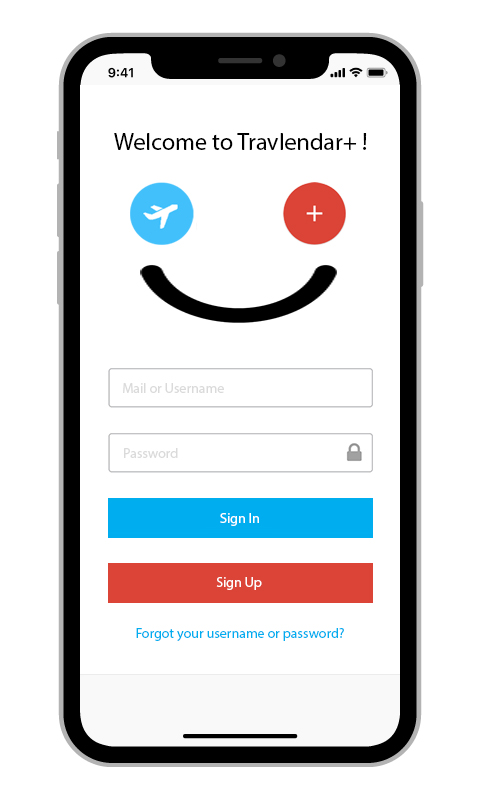
\includegraphics[scale=2.4]{MainMatter/images/ui/login}
\captionof{figure}{Mockup of the login screen}
\end{center}
After downloading the application from the store of the OS. At the first start if the user is not registered, so it is a guest yet, he must sign up. Otherwise he can log in. If he is signing up he will see the registration screen.
\begin{center}
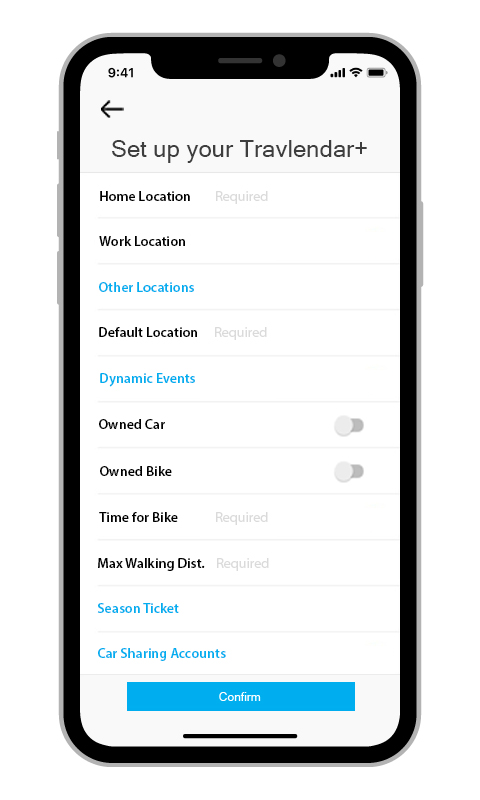
\includegraphics[scale=2.4]{MainMatter/images/ui/firstsetup}
\captionof{figure}{Mockup of the first configuration screen}
\end{center}
The first time the user signs in, the application shows the first setup screen where the user has to insert all his preferences. The light blue texts open other screen where more are given for the specific setting. \\\
Once the application is configured, the first screen that will appear to the user at each startup is the main screen that shows up a calendar, where he can add his events.
\begin{center}
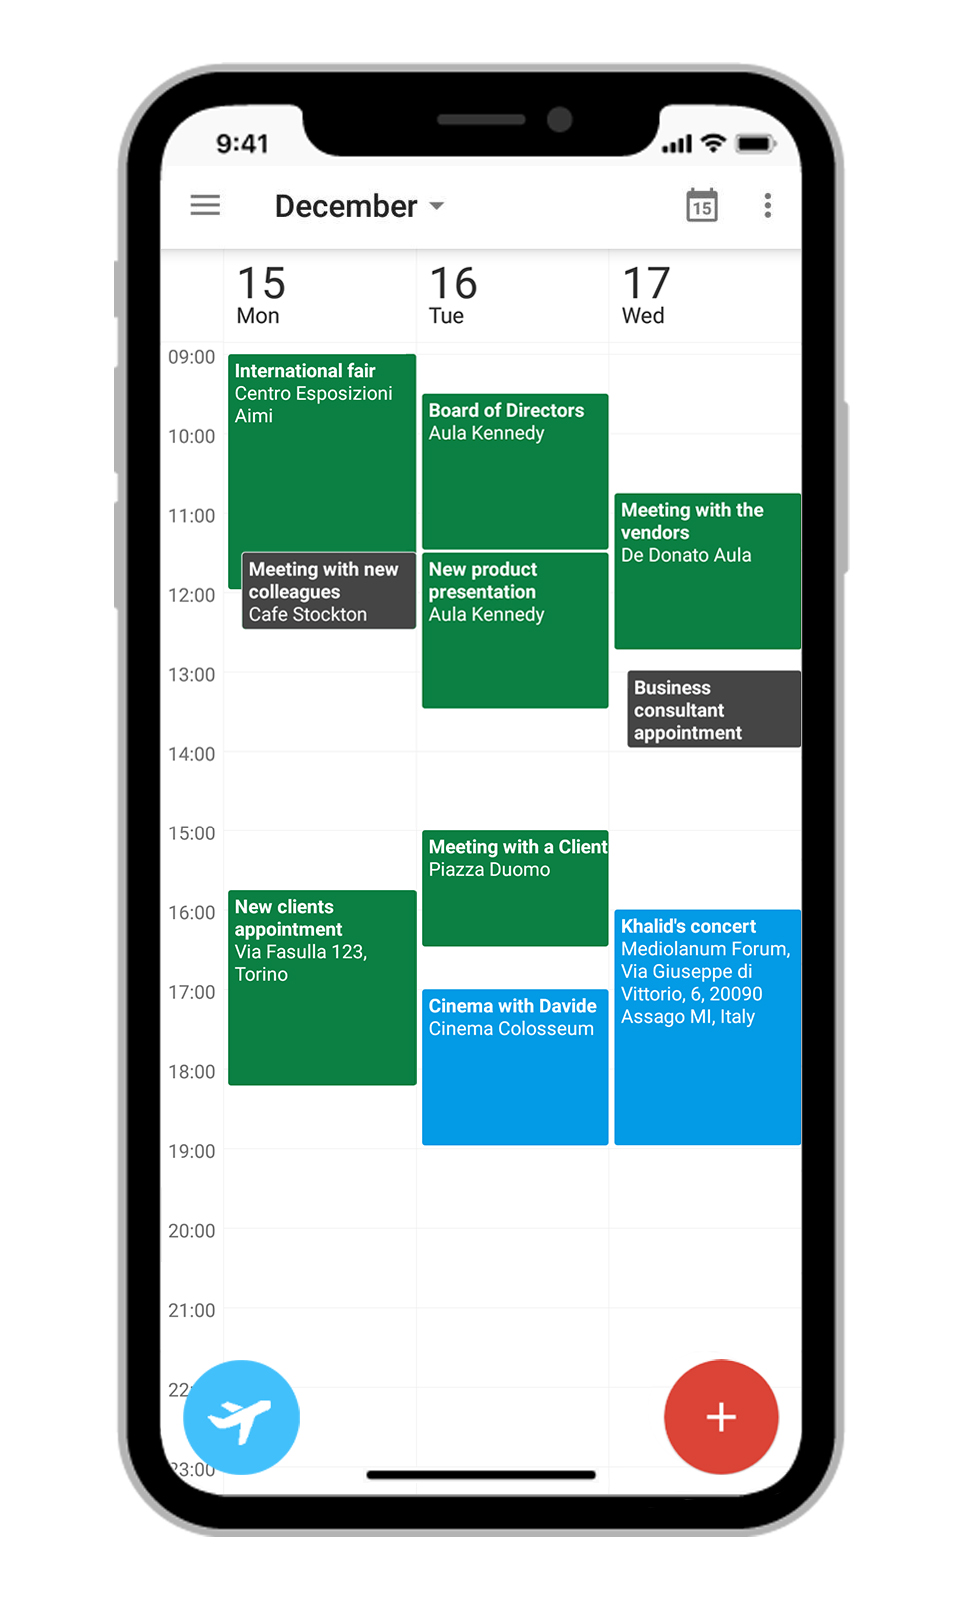
\includegraphics[scale=1.2]{MainMatter/images/ui/calendar}
\captionof{figure}{Mockup of the main screen (calendar)}
\end{center}
The events are the ones in green or blue, some event are not coloured cause are overlapped with others or the user cannot phisically arrive on time for them (the user chooses what event is primary and the application considers it to organize the trips. When the user chooses to add an event pressing the "Add Event" button on the bottom right corner (the red one with a cross on it), the application shows a screen where he can insert the details of it.
\begin{center}
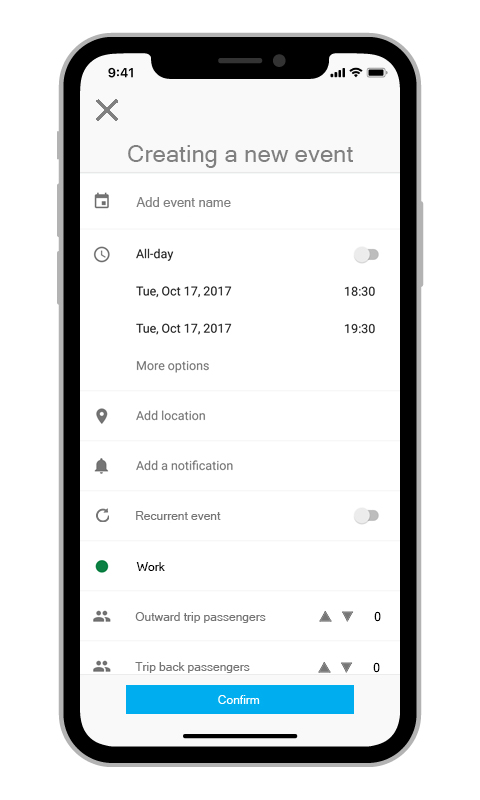
\includegraphics[scale=2.4]{MainMatter/images/ui/newevent}
\captionof{figure}{Mockup of the screen that appears to the user when he has to add an event}
\end{center}
When the main screen is showed by the application, to check the trips between home and an event, or between two events, the user can press the "Trips" button on the bottom left side of the screen (the light blue one with a plane on it) and the main screen will change to show the trips and all the confirmed events will become black and white.
\begin{center}
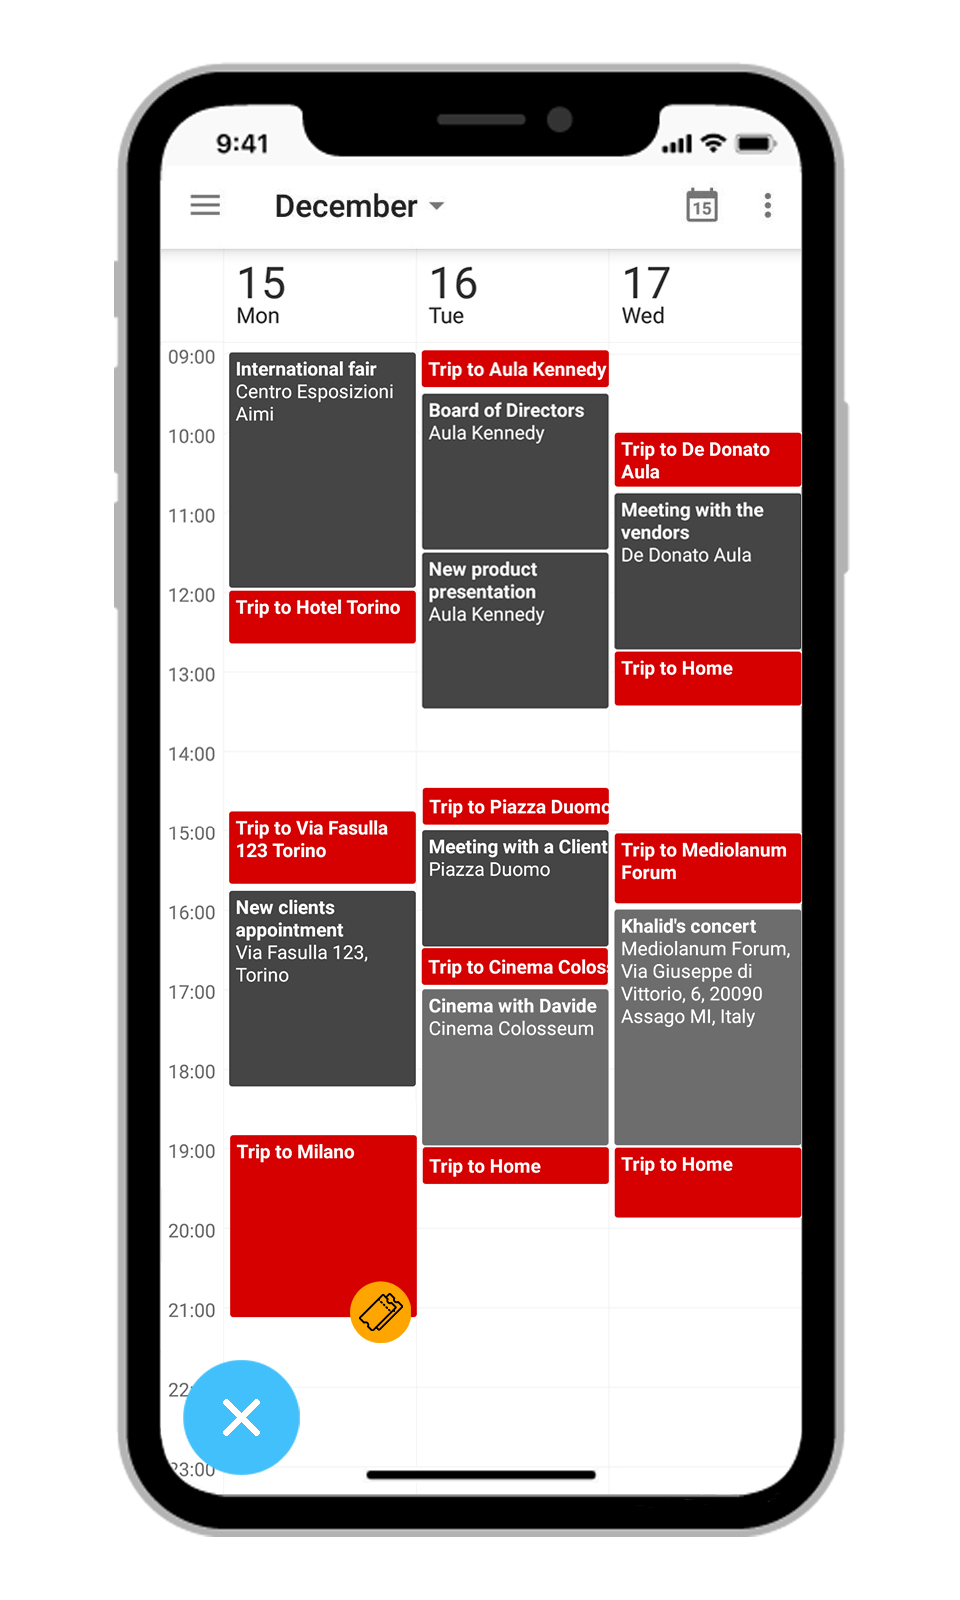
\includegraphics[scale=1.2]{MainMatter/images/ui/tripsscreen}
\captionof{figure}{Mockup of the screen that contains all the trips computed by the application for the user}
\end{center}
When the user taps on a trip he can check the details of it. If a trip presents an orange icon with some tickets on it, the user have to buy some tickets to complete the trip.
\begin{center}
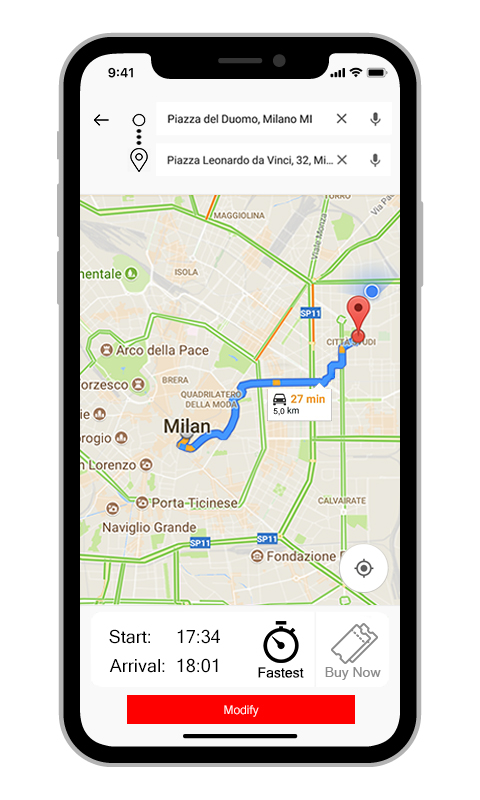
\includegraphics[scale=2.4]{MainMatter/images/ui/journeydetails}
\captionof{figure}{Mockup of the screen that shows the details of a trip}
\end{center}
This screen shows the trip details: the route, the ETA, the time of departure, the time of arrival, the type of trip selected. If some tickets are needed the "Buy Now" button with the tickets on it is grey, but black and it will be clickable. The "Buy Now" is juxtaposed with the "Sharing" button if the trip include some section in which car sharing or bike sharing are used; clicking on the "Bike sharing" or "Car sharing" button will show up a screen with the cars and bike around the user of the various local sharing service. \\
If an user wants to modify a trip, he just have to press "Modify" button and a screen will appear when he can change the trip options.
\begin{center}
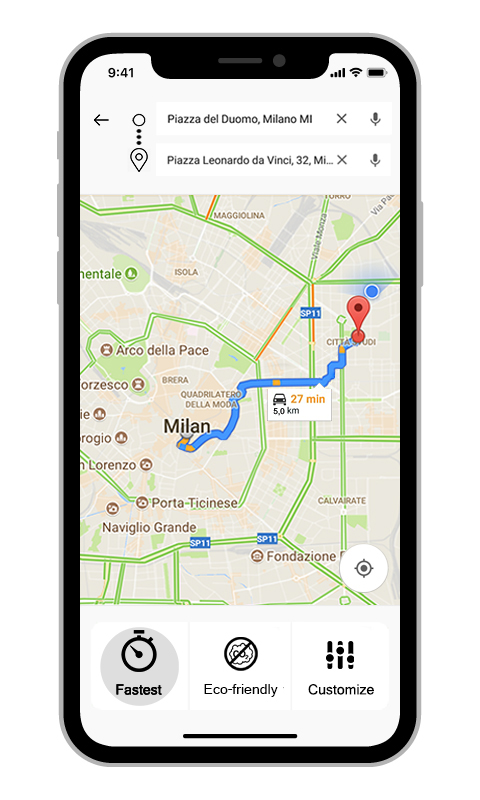
\includegraphics[scale=2.4]{MainMatter/images/ui/journeychoose}
\captionof{figure}{Mockup of the screen where the user can change the trip options}
\end{center}
The system select by default the fastest trip options, but the user can change them. It is also possible to choose a trip that minimize the carbon footprint.
\\
\\
When the application need to communicate messages to the user, while it’s open and the screen is turned on, it will show a pop up, otherwise it will send a push notification to the user.
%
\subsection{Hardware interfaces}
The main hardware interface used by the system is the GPS, it's used in order to correctly position the user in the map. Since the application uses the internet connection, all the hardware required to connect to the internet will be hardware interface for the system.
%
\subsection{Software interfaces}
The mobile application is made up using mainly two Google APIs: Google Maps and Google Calendar. It relies also on other APIs: one for the weather forecast and one for each car sharing, bike sharing service and for the public mobility.
It is developed for the use on the two most common mobile operating systems: Android and iOS.
%
\subsection{Communication interfaces}
The application communicates with the server using the protocol HTTP (port 80).
%
%------------------------------------------------------------------------ %
%
\section{Performance Requirements}
\begin{enumerate}
\item The system must support 500 contemporary requests;
\item 90\% of requests must be processed in less than 3 seconds;
\item 100\% of requests must be processed in less than 10 seconds;
\item There’s no limit on the number of users;
\item Trips solutions are updated daily until the day of the trip, then every hour until half an hour before the trip, finally every minute until the trip begins;
\item The system will compute continuously all the travel options for the different users, but must find a free time spot to answer to new requests.
\end{enumerate}
%
% ------------------------------------------------------------------------ %
%
\section{Design Constraints}
%
\subsection{Standards compliance}
This document follows the IEEE Standard 830-1998 [7] for the format of Software Requirements specifications.
%
\subsection{Hardware limitations}
The user will need a smartphone with at least:
\begin{itemize}
\item 3G connection
\item GPS
\item Enough storage on smartphone
\end{itemize}
%
%
\section{Regulatory policy}
The System asks the User for the permission to acquire, store and use his personal data, and informs him that won't take any responsibility for a use of it that doesn't complies with the local laws and policies, by means of the User agreement's acceptance.
The System under request of the User must delete all his personal data.
%
%
\section{Software System Attributes}
%
\subsection{Reliability}
The system shall have an availability of 99.95\% (“three and a half nines”). It means that the application will have at most a downtime per year of 4.38 hours.
%
\subsection{Availability}
The system will run 24/7 in order to make the user manage his events and the trips between them whenever he wants. Furthermore any kind of update must not stop the normal running of operations.
%
\subsection{Security}
The main security features of the application are:  
\begin{itemize}
\item All the meetings and the trips must be kept private.
\item Enable SSL/TLS encryption protocol for Client-Server communication to protect from internal and external threats, depending on user’s network configuration. Enabling SSL/TLS ensures the confidentiality, authentication, and integrity of session data.
\item Insecure communication channels will lead to a refuse for the client’s request.
\item Passwords must be encrypted, hashed and salted before they could be stored in the databases.
\item Users can access in reading or in writing on only a limited set of data.
\end{itemize}
%
\subsection{Maintainability}
The application code will be well documented to let future developers understand how it work and to make them able to modify it.
%
\subsection{Portability}
The application will be available for the two most common mobile operating systems: Android and iOS.
% ------------------------------------------------------------------------ %


% -----------------------------END------------------------------------- %
